\chapter{p4 = 11 (18 graphs)}
\newpage\begin{figure}
  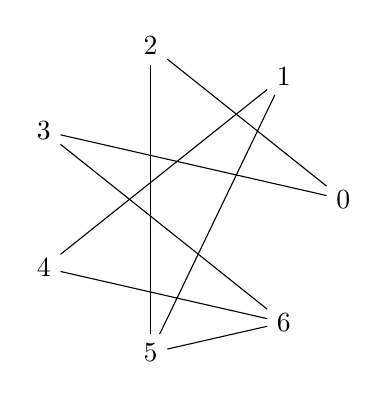
\begin{tikzpicture}
      \draw
        (0.0:2) node (0){0}
        (51.429:2) node (1){1}
        (102.857:2) node (2){2}
        (154.286:2) node (3){3}
        (205.714:2) node (4){4}
        (257.143:2) node (5){5}
        (308.571:2) node (6){6};
      \begin{scope}[-]
        \draw (0) to (2);
        \draw (0) to (3);
        \draw (1) to (4);
        \draw (1) to (5);
        \draw (2) to (5);
        \draw (3) to (6);
        \draw (4) to (6);
        \draw (5) to (6);
      \end{scope}
    \end{tikzpicture}
\end{figure}
\begin{itemize}
\item signature: 011000001100010001011
\item g: Graph with 7 nodes and 8 edges
\item order: 7
\item size: 8
\item max degree: 3
\item degrees: 2,2,2,2,2,3,3
\item is tree: 0
\item is bipartite: 0
\item has bridge: 0
\item is chordal: 0
\item is complete: 0
\item min cycle basis weight: 9
\item min cycle basis size: 2
\item diameter: 3
\item radius: 2
\item is eulerian: 0
\item is planar: 1
\item number of faces: 3
\item is regular: 0
\item p3: 11
\item p4: 11
\item property hash: 4c012f1dfcea1ff35cd24f0575d6479e55fb39e1affc0e4464af049dfcc2526c
\end{itemize}
\newpage
\begin{figure}
  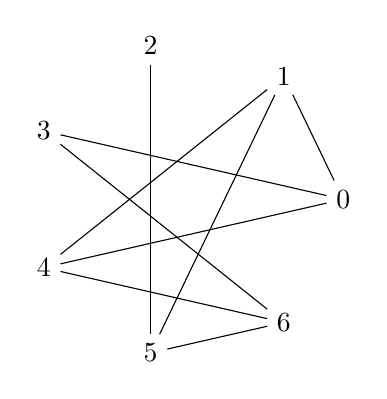
\begin{tikzpicture}
      \draw
        (0.0:2) node (0){0}
        (51.429:2) node (1){1}
        (102.857:2) node (2){2}
        (154.286:2) node (3){3}
        (205.714:2) node (4){4}
        (257.143:2) node (5){5}
        (308.571:2) node (6){6};
      \begin{scope}[-]
        \draw (0) to (1);
        \draw (0) to (3);
        \draw (0) to (4);
        \draw (1) to (4);
        \draw (1) to (5);
        \draw (2) to (5);
        \draw (3) to (6);
        \draw (4) to (6);
        \draw (5) to (6);
      \end{scope}
    \end{tikzpicture}
\end{figure}
\begin{itemize}
\item signature: 101100001100010001011
\item g: Graph with 7 nodes and 9 edges
\item order: 7
\item size: 9
\item max degree: 3
\item degrees: 1,2,3,3,3,3,3
\item is tree: 0
\item is bipartite: 0
\item has bridge: 1
\item is chordal: 0
\item is complete: 0
\item min cycle basis weight: 11
\item min cycle basis size: 3
\item diameter: 3
\item radius: 2
\item is eulerian: 0
\item is planar: 1
\item number of faces: 4
\item is regular: 0
\item p3: 13
\item p4: 11
\item property hash: 109ca8d622e4bb66e54eabe8cb198b8ee032280a945190801936d623332c4562
\end{itemize}
\newpage
\begin{figure}
  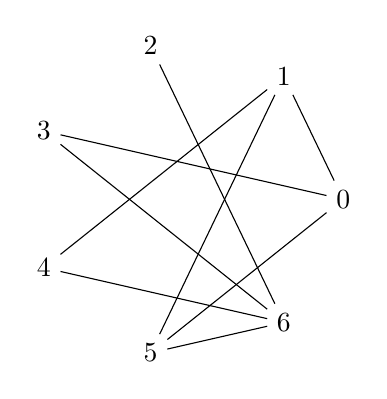
\begin{tikzpicture}
      \draw
        (0.0:2) node (0){0}
        (51.429:2) node (1){1}
        (102.857:2) node (2){2}
        (154.286:2) node (3){3}
        (205.714:2) node (4){4}
        (257.143:2) node (5){5}
        (308.571:2) node (6){6};
      \begin{scope}[-]
        \draw (0) to (1);
        \draw (0) to (3);
        \draw (0) to (5);
        \draw (1) to (4);
        \draw (1) to (5);
        \draw (2) to (6);
        \draw (3) to (6);
        \draw (4) to (6);
        \draw (5) to (6);
      \end{scope}
    \end{tikzpicture}
\end{figure}
\begin{itemize}
\item signature: 101010001100001001011
\item g: Graph with 7 nodes and 9 edges
\item order: 7
\item size: 9
\item max degree: 4
\item degrees: 1,2,2,3,3,3,4
\item is tree: 0
\item is bipartite: 0
\item has bridge: 1
\item is chordal: 0
\item is complete: 0
\item min cycle basis weight: 11
\item min cycle basis size: 3
\item diameter: 3
\item radius: 2
\item is eulerian: 0
\item is planar: 1
\item number of faces: 4
\item is regular: 0
\item p3: 14
\item p4: 11
\item property hash: 1f551845db55c08435aadc413e0219c6e3d24cd70f9240d3fc14bf24146ea903
\end{itemize}
\newpage
\begin{figure}
  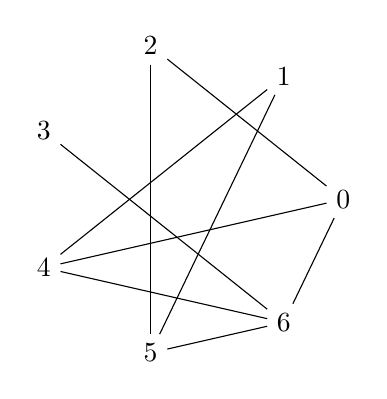
\begin{tikzpicture}
      \draw
        (0.0:2) node (0){0}
        (51.429:2) node (1){1}
        (102.857:2) node (2){2}
        (154.286:2) node (3){3}
        (205.714:2) node (4){4}
        (257.143:2) node (5){5}
        (308.571:2) node (6){6};
      \begin{scope}[-]
        \draw (0) to (2);
        \draw (0) to (4);
        \draw (0) to (6);
        \draw (1) to (4);
        \draw (1) to (5);
        \draw (2) to (5);
        \draw (3) to (6);
        \draw (4) to (6);
        \draw (5) to (6);
      \end{scope}
    \end{tikzpicture}
\end{figure}
\begin{itemize}
\item signature: 010101001100010001011
\item g: Graph with 7 nodes and 9 edges
\item order: 7
\item size: 9
\item max degree: 4
\item degrees: 1,2,2,3,3,3,4
\item is tree: 0
\item is bipartite: 0
\item has bridge: 1
\item is chordal: 0
\item is complete: 0
\item min cycle basis weight: 11
\item min cycle basis size: 3
\item diameter: 3
\item radius: 2
\item is eulerian: 0
\item is planar: 1
\item number of faces: 4
\item is regular: 0
\item p3: 14
\item p4: 11
\item property hash: 1f551845db55c08435aadc413e0219c6e3d24cd70f9240d3fc14bf24146ea903
\end{itemize}
\newpage
\begin{figure}
  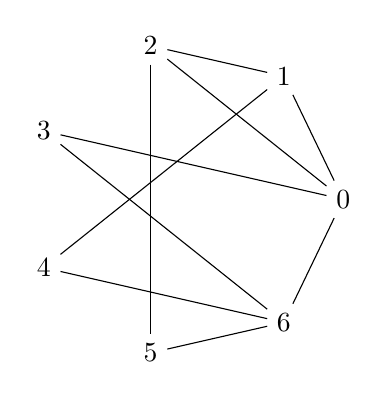
\begin{tikzpicture}
      \draw
        (0.0:2) node (0){0}
        (51.429:2) node (1){1}
        (102.857:2) node (2){2}
        (154.286:2) node (3){3}
        (205.714:2) node (4){4}
        (257.143:2) node (5){5}
        (308.571:2) node (6){6};
      \begin{scope}[-]
        \draw (0) to (1);
        \draw (0) to (2);
        \draw (0) to (3);
        \draw (0) to (6);
        \draw (1) to (2);
        \draw (1) to (4);
        \draw (2) to (5);
        \draw (3) to (6);
        \draw (4) to (6);
        \draw (5) to (6);
      \end{scope}
    \end{tikzpicture}
\end{figure}
\begin{itemize}
\item signature: 111001101000010001011
\item g: Graph with 7 nodes and 10 edges
\item order: 7
\item size: 10
\item max degree: 4
\item degrees: 2,2,2,3,3,4,4
\item is tree: 0
\item is bipartite: 0
\item has bridge: 0
\item is chordal: 0
\item is complete: 0
\item min cycle basis weight: 14
\item min cycle basis size: 4
\item diameter: 2
\item radius: 2
\item is eulerian: 0
\item is planar: 1
\item number of faces: 5
\item is regular: 0
\item p3: 15
\item p4: 11
\item property hash: 6c3de26268c5a89170effac632c778b7349e1b28a3fe1b3191f0ba0e94093685
\end{itemize}
\newpage
\begin{figure}
  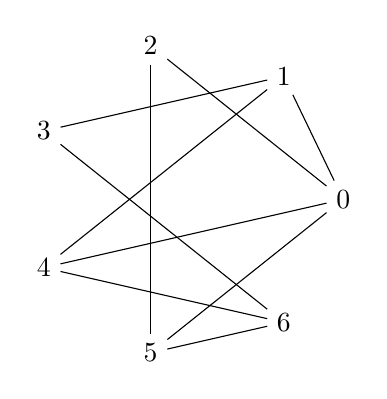
\begin{tikzpicture}
      \draw
        (0.0:2) node (0){0}
        (51.429:2) node (1){1}
        (102.857:2) node (2){2}
        (154.286:2) node (3){3}
        (205.714:2) node (4){4}
        (257.143:2) node (5){5}
        (308.571:2) node (6){6};
      \begin{scope}[-]
        \draw (0) to (1);
        \draw (0) to (2);
        \draw (0) to (4);
        \draw (0) to (5);
        \draw (1) to (3);
        \draw (1) to (4);
        \draw (2) to (5);
        \draw (3) to (6);
        \draw (4) to (6);
        \draw (5) to (6);
      \end{scope}
    \end{tikzpicture}
\end{figure}
\begin{itemize}
\item signature: 110110011000010001011
\item g: Graph with 7 nodes and 10 edges
\item order: 7
\item size: 10
\item max degree: 4
\item degrees: 2,2,3,3,3,3,4
\item is tree: 0
\item is bipartite: 0
\item has bridge: 0
\item is chordal: 0
\item is complete: 0
\item min cycle basis weight: 14
\item min cycle basis size: 4
\item diameter: 3
\item radius: 2
\item is eulerian: 0
\item is planar: 1
\item number of faces: 5
\item is regular: 0
\item p3: 14
\item p4: 11
\item property hash: 20b5e66ee517873a20343d96186c991179a8448715c2f7acb0f6734ed4455e34
\end{itemize}
\newpage
\begin{figure}
  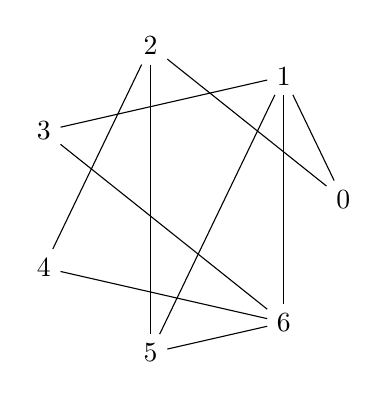
\begin{tikzpicture}
      \draw
        (0.0:2) node (0){0}
        (51.429:2) node (1){1}
        (102.857:2) node (2){2}
        (154.286:2) node (3){3}
        (205.714:2) node (4){4}
        (257.143:2) node (5){5}
        (308.571:2) node (6){6};
      \begin{scope}[-]
        \draw (0) to (1);
        \draw (0) to (2);
        \draw (1) to (3);
        \draw (1) to (5);
        \draw (1) to (6);
        \draw (2) to (4);
        \draw (2) to (5);
        \draw (3) to (6);
        \draw (4) to (6);
        \draw (5) to (6);
      \end{scope}
    \end{tikzpicture}
\end{figure}
\begin{itemize}
\item signature: 110000010110110001011
\item g: Graph with 7 nodes and 10 edges
\item order: 7
\item size: 10
\item max degree: 4
\item degrees: 2,2,2,3,3,4,4
\item is tree: 0
\item is bipartite: 0
\item has bridge: 0
\item is chordal: 0
\item is complete: 0
\item min cycle basis weight: 14
\item min cycle basis size: 4
\item diameter: 3
\item radius: 2
\item is eulerian: 0
\item is planar: 1
\item number of faces: 5
\item is regular: 0
\item p3: 15
\item p4: 11
\item property hash: 6f5ffd110bd7d2c3cafcdb0da74f25ed1ebc646e8883da9c852ab0b312177c25
\end{itemize}
\newpage
\begin{figure}
  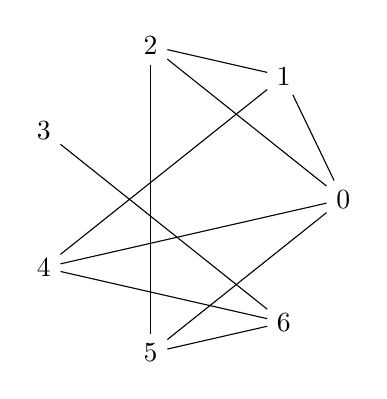
\begin{tikzpicture}
      \draw
        (0.0:2) node (0){0}
        (51.429:2) node (1){1}
        (102.857:2) node (2){2}
        (154.286:2) node (3){3}
        (205.714:2) node (4){4}
        (257.143:2) node (5){5}
        (308.571:2) node (6){6};
      \begin{scope}[-]
        \draw (0) to (1);
        \draw (0) to (2);
        \draw (0) to (4);
        \draw (0) to (5);
        \draw (1) to (2);
        \draw (1) to (4);
        \draw (2) to (5);
        \draw (3) to (6);
        \draw (4) to (6);
        \draw (5) to (6);
      \end{scope}
    \end{tikzpicture}
\end{figure}
\begin{itemize}
\item signature: 110110101000010001011
\item g: Graph with 7 nodes and 10 edges
\item order: 7
\item size: 10
\item max degree: 4
\item degrees: 1,3,3,3,3,3,4
\item is tree: 0
\item is bipartite: 0
\item has bridge: 1
\item is chordal: 0
\item is complete: 0
\item min cycle basis weight: 13
\item min cycle basis size: 4
\item diameter: 3
\item radius: 2
\item is eulerian: 0
\item is planar: 1
\item number of faces: 5
\item is regular: 0
\item p3: 12
\item p4: 11
\item property hash: 1d95e4848f56b5ea95449bec649667c37c43d95b63c02750df08bc9dc17ca9df
\end{itemize}
\newpage
\begin{figure}
  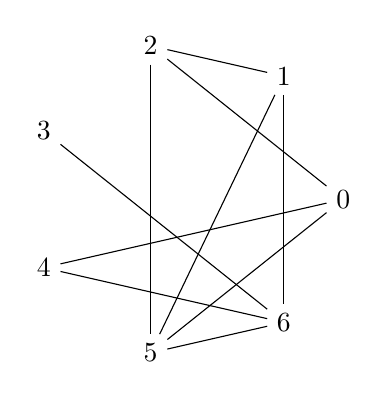
\begin{tikzpicture}
      \draw
        (0.0:2) node (0){0}
        (51.429:2) node (1){1}
        (102.857:2) node (2){2}
        (154.286:2) node (3){3}
        (205.714:2) node (4){4}
        (257.143:2) node (5){5}
        (308.571:2) node (6){6};
      \begin{scope}[-]
        \draw (0) to (2);
        \draw (0) to (4);
        \draw (0) to (5);
        \draw (1) to (2);
        \draw (1) to (5);
        \draw (1) to (6);
        \draw (2) to (5);
        \draw (3) to (6);
        \draw (4) to (6);
        \draw (5) to (6);
      \end{scope}
    \end{tikzpicture}
\end{figure}
\begin{itemize}
\item signature: 010110100110010001011
\item g: Graph with 7 nodes and 10 edges
\item order: 7
\item size: 10
\item max degree: 4
\item degrees: 1,2,3,3,3,4,4
\item is tree: 0
\item is bipartite: 0
\item has bridge: 1
\item is chordal: 0
\item is complete: 0
\item min cycle basis weight: 13
\item min cycle basis size: 4
\item diameter: 3
\item radius: 2
\item is eulerian: 0
\item is planar: 1
\item number of faces: 5
\item is regular: 0
\item p3: 13
\item p4: 11
\item property hash: 0fb2de2ecee9de1df36d0f43f317d78cf3388117134be9cd154354b3e7aca40b
\end{itemize}
\newpage
\begin{figure}
  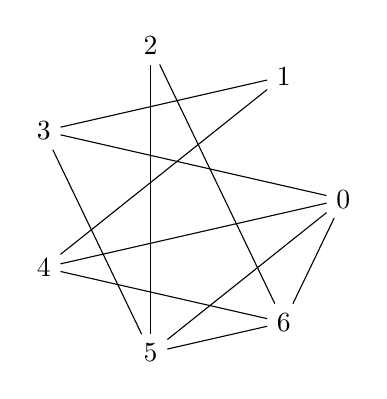
\begin{tikzpicture}
      \draw
        (0.0:2) node (0){0}
        (51.429:2) node (1){1}
        (102.857:2) node (2){2}
        (154.286:2) node (3){3}
        (205.714:2) node (4){4}
        (257.143:2) node (5){5}
        (308.571:2) node (6){6};
      \begin{scope}[-]
        \draw (0) to (3);
        \draw (0) to (4);
        \draw (0) to (5);
        \draw (0) to (6);
        \draw (1) to (3);
        \draw (1) to (4);
        \draw (2) to (5);
        \draw (2) to (6);
        \draw (3) to (5);
        \draw (4) to (6);
        \draw (5) to (6);
      \end{scope}
    \end{tikzpicture}
\end{figure}
\begin{itemize}
\item signature: 001111011000011010011
\item g: Graph with 7 nodes and 11 edges
\item order: 7
\item size: 11
\item max degree: 4
\item degrees: 2,2,3,3,4,4,4
\item is tree: 0
\item is bipartite: 0
\item has bridge: 0
\item is chordal: 0
\item is complete: 0
\item min cycle basis weight: 16
\item min cycle basis size: 5
\item diameter: 3
\item radius: 2
\item is eulerian: 0
\item is planar: 1
\item number of faces: 6
\item is regular: 0
\item p3: 14
\item p4: 11
\item property hash: 8787ad6c1473d3b16ad0dc5a3a9117d9a5518c6f3e345323d1b0b223385edaec
\end{itemize}
\newpage
\begin{figure}
  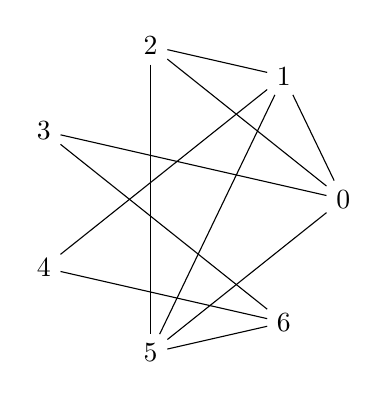
\begin{tikzpicture}
      \draw
        (0.0:2) node (0){0}
        (51.429:2) node (1){1}
        (102.857:2) node (2){2}
        (154.286:2) node (3){3}
        (205.714:2) node (4){4}
        (257.143:2) node (5){5}
        (308.571:2) node (6){6};
      \begin{scope}[-]
        \draw (0) to (1);
        \draw (0) to (2);
        \draw (0) to (3);
        \draw (0) to (5);
        \draw (1) to (2);
        \draw (1) to (4);
        \draw (1) to (5);
        \draw (2) to (5);
        \draw (3) to (6);
        \draw (4) to (6);
        \draw (5) to (6);
      \end{scope}
    \end{tikzpicture}
\end{figure}
\begin{itemize}
\item signature: 111010101100010001011
\item g: Graph with 7 nodes and 11 edges
\item order: 7
\item size: 11
\item max degree: 4
\item degrees: 2,2,3,3,4,4,4
\item is tree: 0
\item is bipartite: 0
\item has bridge: 0
\item is chordal: 0
\item is complete: 0
\item min cycle basis weight: 17
\item min cycle basis size: 5
\item diameter: 2
\item radius: 2
\item is eulerian: 0
\item is planar: 1
\item number of faces: 6
\item is regular: 0
\item p3: 14
\item p4: 11
\item property hash: 4b8b43c7e021bc03d1a9828c6337f921bc490e0f9af3c029f45a1f281de5984f
\end{itemize}
\newpage
\begin{figure}
  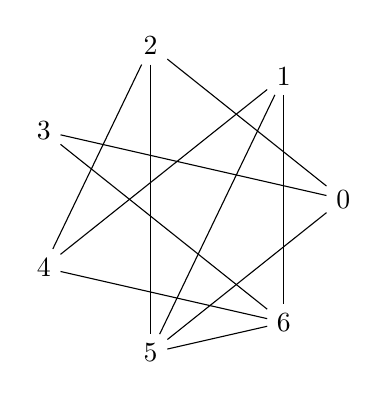
\begin{tikzpicture}
      \draw
        (0.0:2) node (0){0}
        (51.429:2) node (1){1}
        (102.857:2) node (2){2}
        (154.286:2) node (3){3}
        (205.714:2) node (4){4}
        (257.143:2) node (5){5}
        (308.571:2) node (6){6};
      \begin{scope}[-]
        \draw (0) to (2);
        \draw (0) to (3);
        \draw (0) to (5);
        \draw (1) to (4);
        \draw (1) to (5);
        \draw (1) to (6);
        \draw (2) to (4);
        \draw (2) to (5);
        \draw (3) to (6);
        \draw (4) to (6);
        \draw (5) to (6);
      \end{scope}
    \end{tikzpicture}
\end{figure}
\begin{itemize}
\item signature: 011010001110110001011
\item g: Graph with 7 nodes and 11 edges
\item order: 7
\item size: 11
\item max degree: 4
\item degrees: 2,3,3,3,3,4,4
\item is tree: 0
\item is bipartite: 0
\item has bridge: 0
\item is chordal: 0
\item is complete: 0
\item min cycle basis weight: 17
\item min cycle basis size: 5
\item diameter: 2
\item radius: 2
\item is eulerian: 0
\item is planar: 1
\item number of faces: 6
\item is regular: 0
\item p3: 16
\item p4: 11
\item property hash: eac19f1ce288f30328b5578394ea0da8605c772f752ac2018eee44bf9339ec26
\end{itemize}
\newpage
\begin{figure}
  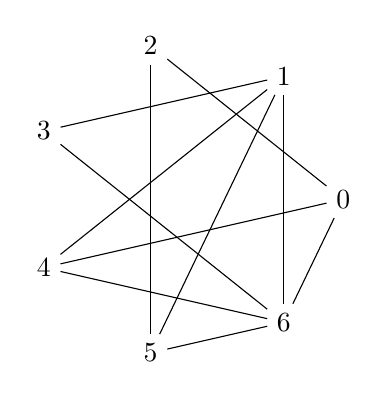
\begin{tikzpicture}
      \draw
        (0.0:2) node (0){0}
        (51.429:2) node (1){1}
        (102.857:2) node (2){2}
        (154.286:2) node (3){3}
        (205.714:2) node (4){4}
        (257.143:2) node (5){5}
        (308.571:2) node (6){6};
      \begin{scope}[-]
        \draw (0) to (2);
        \draw (0) to (4);
        \draw (0) to (6);
        \draw (1) to (3);
        \draw (1) to (4);
        \draw (1) to (5);
        \draw (1) to (6);
        \draw (2) to (5);
        \draw (3) to (6);
        \draw (4) to (6);
        \draw (5) to (6);
      \end{scope}
    \end{tikzpicture}
\end{figure}
\begin{itemize}
\item signature: 010101011110010001011
\item g: Graph with 7 nodes and 11 edges
\item order: 7
\item size: 11
\item max degree: 5
\item degrees: 2,2,3,3,3,4,5
\item is tree: 0
\item is bipartite: 0
\item has bridge: 0
\item is chordal: 0
\item is complete: 0
\item min cycle basis weight: 16
\item min cycle basis size: 5
\item diameter: 3
\item radius: 2
\item is eulerian: 0
\item is planar: 1
\item number of faces: 6
\item is regular: 0
\item p3: 15
\item p4: 11
\item property hash: 55c594614f91400501e83b07c4573e51d16346ef2c31aae89e2a7b2ff77b8d08
\end{itemize}
\newpage
\begin{figure}
  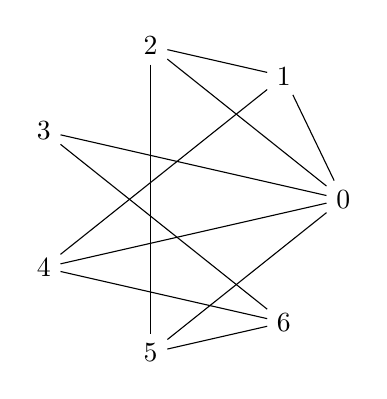
\begin{tikzpicture}
      \draw
        (0.0:2) node (0){0}
        (51.429:2) node (1){1}
        (102.857:2) node (2){2}
        (154.286:2) node (3){3}
        (205.714:2) node (4){4}
        (257.143:2) node (5){5}
        (308.571:2) node (6){6};
      \begin{scope}[-]
        \draw (0) to (1);
        \draw (0) to (2);
        \draw (0) to (3);
        \draw (0) to (4);
        \draw (0) to (5);
        \draw (1) to (2);
        \draw (1) to (4);
        \draw (2) to (5);
        \draw (3) to (6);
        \draw (4) to (6);
        \draw (5) to (6);
      \end{scope}
    \end{tikzpicture}
\end{figure}
\begin{itemize}
\item signature: 111110101000010001011
\item g: Graph with 7 nodes and 11 edges
\item order: 7
\item size: 11
\item max degree: 5
\item degrees: 2,3,3,3,3,3,5
\item is tree: 0
\item is bipartite: 0
\item has bridge: 0
\item is chordal: 0
\item is complete: 0
\item min cycle basis weight: 17
\item min cycle basis size: 5
\item diameter: 2
\item radius: 2
\item is eulerian: 0
\item is planar: 1
\item number of faces: 6
\item is regular: 0
\item p3: 17
\item p4: 11
\item property hash: 39a7623b081b28e49fa20d1babf996aa50813f5134c72795b26ac85a29f10846
\end{itemize}
\newpage
\begin{figure}
  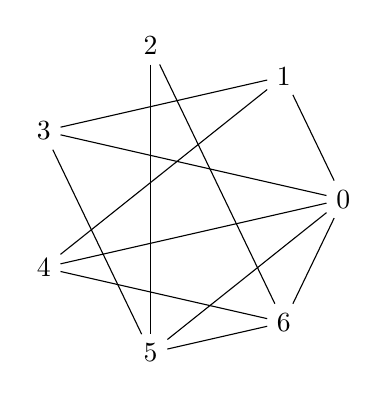
\begin{tikzpicture}
      \draw
        (0.0:2) node (0){0}
        (51.429:2) node (1){1}
        (102.857:2) node (2){2}
        (154.286:2) node (3){3}
        (205.714:2) node (4){4}
        (257.143:2) node (5){5}
        (308.571:2) node (6){6};
      \begin{scope}[-]
        \draw (0) to (1);
        \draw (0) to (3);
        \draw (0) to (4);
        \draw (0) to (5);
        \draw (0) to (6);
        \draw (1) to (3);
        \draw (1) to (4);
        \draw (2) to (5);
        \draw (2) to (6);
        \draw (3) to (5);
        \draw (4) to (6);
        \draw (5) to (6);
      \end{scope}
    \end{tikzpicture}
\end{figure}
\begin{itemize}
\item signature: 101111011000011010011
\item g: Graph with 7 nodes and 12 edges
\item order: 7
\item size: 12
\item max degree: 5
\item degrees: 2,3,3,3,4,4,5
\item is tree: 0
\item is bipartite: 0
\item has bridge: 0
\item is chordal: 0
\item is complete: 0
\item min cycle basis weight: 18
\item min cycle basis size: 6
\item diameter: 3
\item radius: 2
\item is eulerian: 0
\item is planar: 1
\item number of faces: 7
\item is regular: 0
\item p3: 14
\item p4: 11
\item property hash: 6a6932349138da8a074e37d3dcda357b8a4ac0a7e6b26584da9ba07b6368f7cf
\end{itemize}
\newpage
\begin{figure}
  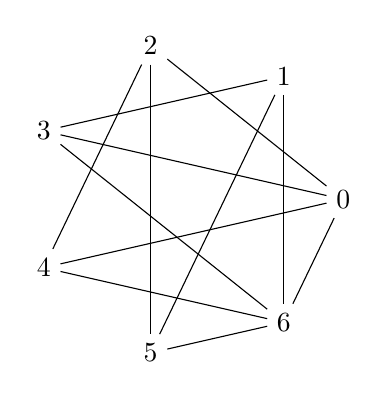
\begin{tikzpicture}
      \draw
        (0.0:2) node (0){0}
        (51.429:2) node (1){1}
        (102.857:2) node (2){2}
        (154.286:2) node (3){3}
        (205.714:2) node (4){4}
        (257.143:2) node (5){5}
        (308.571:2) node (6){6};
      \begin{scope}[-]
        \draw (0) to (2);
        \draw (0) to (3);
        \draw (0) to (4);
        \draw (0) to (6);
        \draw (1) to (3);
        \draw (1) to (5);
        \draw (1) to (6);
        \draw (2) to (4);
        \draw (2) to (5);
        \draw (3) to (6);
        \draw (4) to (6);
        \draw (5) to (6);
      \end{scope}
    \end{tikzpicture}
\end{figure}
\begin{itemize}
\item signature: 011101010110110001011
\item g: Graph with 7 nodes and 12 edges
\item order: 7
\item size: 12
\item max degree: 5
\item degrees: 3,3,3,3,3,4,5
\item is tree: 0
\item is bipartite: 0
\item has bridge: 0
\item is chordal: 0
\item is complete: 0
\item min cycle basis weight: 19
\item min cycle basis size: 6
\item diameter: 2
\item radius: 2
\item is eulerian: 0
\item is planar: 1
\item number of faces: 7
\item is regular: 0
\item p3: 16
\item p4: 11
\item property hash: f7529b552fa9b1447f7da68f9b4459a07b085791e26cf54b7fc2e4289c9ce5be
\end{itemize}
\newpage
\begin{figure}
  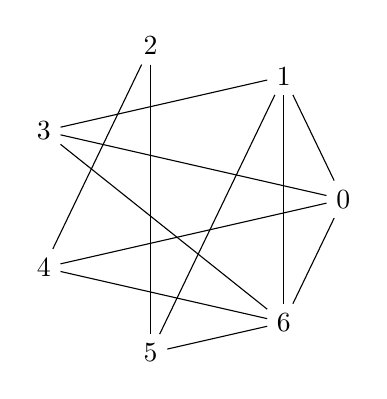
\begin{tikzpicture}
      \draw
        (0.0:2) node (0){0}
        (51.429:2) node (1){1}
        (102.857:2) node (2){2}
        (154.286:2) node (3){3}
        (205.714:2) node (4){4}
        (257.143:2) node (5){5}
        (308.571:2) node (6){6};
      \begin{scope}[-]
        \draw (0) to (1);
        \draw (0) to (3);
        \draw (0) to (4);
        \draw (0) to (6);
        \draw (1) to (3);
        \draw (1) to (5);
        \draw (1) to (6);
        \draw (2) to (4);
        \draw (2) to (5);
        \draw (3) to (6);
        \draw (4) to (6);
        \draw (5) to (6);
      \end{scope}
    \end{tikzpicture}
\end{figure}
\begin{itemize}
\item signature: 101101010110110001011
\item g: Graph with 7 nodes and 12 edges
\item order: 7
\item size: 12
\item max degree: 5
\item degrees: 2,3,3,3,4,4,5
\item is tree: 0
\item is bipartite: 0
\item has bridge: 0
\item is chordal: 0
\item is complete: 0
\item min cycle basis weight: 19
\item min cycle basis size: 6
\item diameter: 3
\item radius: 2
\item is eulerian: 0
\item is planar: 1
\item number of faces: 7
\item is regular: 0
\item p3: 14
\item p4: 11
\item property hash: 9ed1a6f86ea11080c34f44a1c253e1a14772ed899ef9d02a2c4c1271d07820d9
\end{itemize}
\newpage
\begin{figure}
  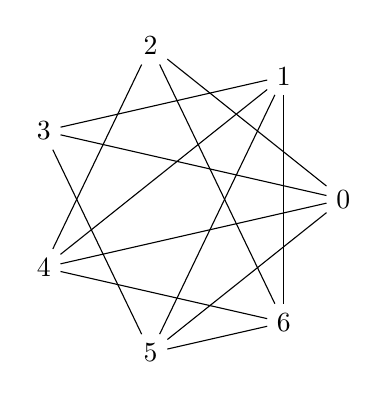
\begin{tikzpicture}
      \draw
        (0.0:2) node (0){0}
        (51.429:2) node (1){1}
        (102.857:2) node (2){2}
        (154.286:2) node (3){3}
        (205.714:2) node (4){4}
        (257.143:2) node (5){5}
        (308.571:2) node (6){6};
      \begin{scope}[-]
        \draw (0) to (2);
        \draw (0) to (3);
        \draw (0) to (4);
        \draw (0) to (5);
        \draw (1) to (3);
        \draw (1) to (4);
        \draw (1) to (5);
        \draw (1) to (6);
        \draw (2) to (4);
        \draw (2) to (6);
        \draw (3) to (5);
        \draw (4) to (6);
        \draw (5) to (6);
      \end{scope}
    \end{tikzpicture}
\end{figure}
\begin{itemize}
\item signature: 011110011110101010011
\item g: Graph with 7 nodes and 13 edges
\item order: 7
\item size: 13
\item max degree: 4
\item degrees: 3,3,4,4,4,4,4
\item is tree: 0
\item is bipartite: 0
\item has bridge: 0
\item is chordal: 0
\item is complete: 0
\item min cycle basis weight: 22
\item min cycle basis size: 7
\item diameter: 2
\item radius: 2
\item is eulerian: 0
\item is planar: 1
\item number of faces: 8
\item is regular: 0
\item p3: 18
\item p4: 11
\item property hash: 3788ddb30cfa31827d87e9d7724ee52abed9f61bb758f7ffd87d0efd6d619041
\end{itemize}
\newpage
